\documentclass[titlepage]{scrartcl}
\usepackage[czech, english]{babel}
\usepackage{amsmath}
\usepackage{graphicx}

\title{Anderson.NET User Documentation\thanks{written for version 0.1.0}}
\author{Václav Luňák}
\begin{document}
\maketitle
\tableofcontents
\pagebreak
\section{General notes}
\subsection{Program dependencies}
As of now, Anderson.NET can only be run on Windows. In addition, you must have the .NET Framework Runtime (version 4.7 or higher) installed. In newer Windows versions, this is installed by default as part of the operating system.\footnote{https://docs.microsoft.com/dotnet/framework/migration-guide/how-to-determine-which-versions-are-installed}

\subsection{Program structure}
The program consists of three main views. A user operating the program will navigate between these views as they use the application, with most time spent in the user view. Detailed description of each view and a guide to operate them is included in the following sections. 

\subsection{Usability warning}
While Anderson.NET is usable in its current form for basic function, it is by no means feature complete. If you feel a particular feature is either missing from the program or not working correctly, please open an issue in the project's repository.\footnote{https://www.github.com/lunakv/Anderson.NET/issues}

As of now, the application window is fixed in size and not allowed to resize or maximize. Minimization is possible.

\section{Installation}
\subsection{Download}
The latest installer is available for download from the Releases page in the project's repository.\footnote{https://www.github.com/lunakv/Anderson.NET/releases}

\subsection{Install}
To install Anderson.NET, simply run the downloaded installer and follow the provided instructions. This will install the application to your specified location as well as add a shortcut to your Start menu.

While any user can run the application, installing it requires administrator privileges on the host system.

\subsection{Uninstall}
You can uninstall Anderson.NET from the "Add or remove programs" section of the system settings, or by rerunning the installer and selecting Remove Anderson.NET.

\section{Title view}
\subsection{Reference} 
\begin{center}
    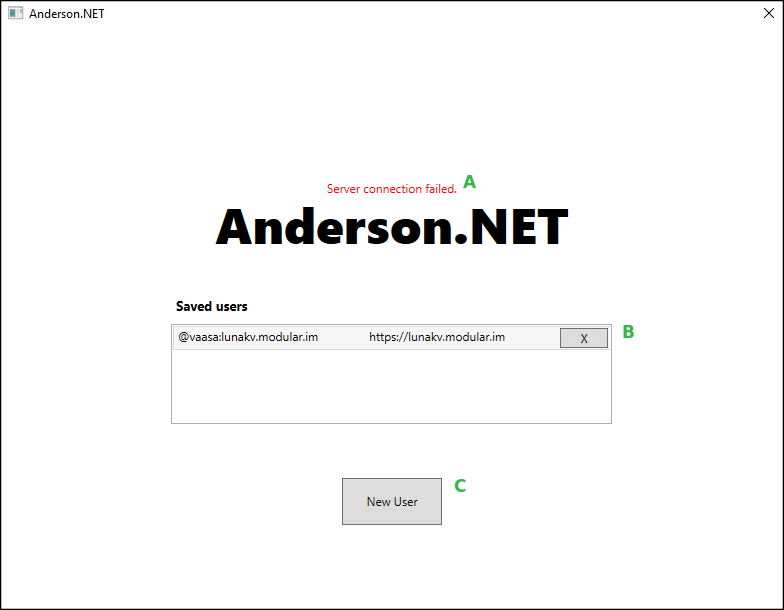
\includegraphics[width=410pt]{title-window.png} 
\end{center}

\subsection{Description}
This is the first view you will see when opening the application. Apart from the title, it contains three main elements.

The error message filed (A) is hidden by default and displays useful information to the user when necessary.

The list of saved users (B) contains all saved logins from all servers in this application. Clicking on an item in this list directly log in the selected user. To delete a saved login, click the "X" button next to the appropriate entry. This list is saved between application sessions.

The New User button (C) takes you to the login view, where you can log in as a user not shown in the list above.
\section{Login view}
\subsection{Reference}
\begin{center}
    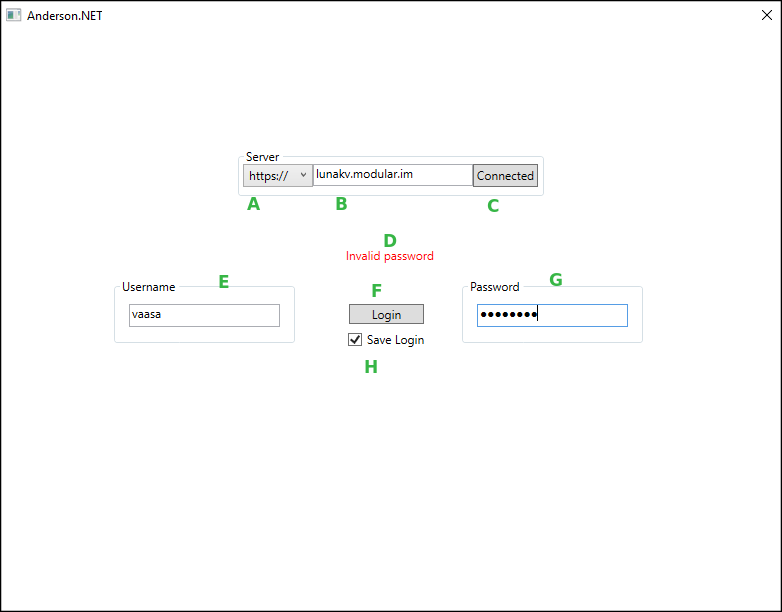
\includegraphics[width=410pt]{login-window.png}
\end{center}

\subsection{Connecting to a server}
In order to log in, you must first connect the application to your home server. First, choose a URL prefix (A). Right now, "https://" and "http://" are supported, with "https://" being the recommended option if available. 

Then, fill out the address of your server to the server field (B). This field can be used to specify ports as well, so "matrix.org:443" is an example of a valid entry (when using the "https://" prefix). 

After that, click the Connect button (C) to attempt connection with the specified server. This button also shows the status of the current connection.

\subsection{Logging in}
After you've successfully connected to a server, as indicated by button (C), enter your username and password into the fields (E) and (G) respectively. If you would like to add these credentials to the list of saved users in the title view, check the "Save Login" checkbox (H). Then, click the "Login" button (F) to attempt login with the connected server.

If any part of this process is unsuccessful, a message will be displayed in the error message area (D). After a successful login, you will be transferred to the user view.

\section{User view}
\subsection{Reference}
\begin{center}
    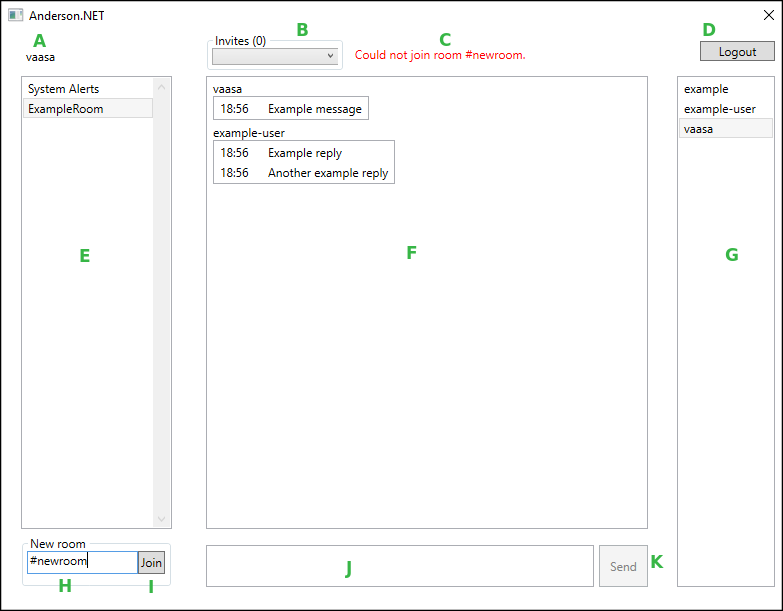
\includegraphics[width=410px]{user-window.png}
\end{center}

\subsection{Overview}
This is the main view of the application. The top left shows the current user's name, under which is the list of all the rooms the user has joined (E) and a field for joining public rooms (H). On the right you can see the logout button (D) and a list of users connected to the active room (G). The middle is the main working area, with a window displaying sent messages (F), a field for sending new messages (J), a list of pending invites (B) and the error message area (C).

\subsection{Selecting a room}
Clicking on a room in the list of joined rooms (E) will select it as the active room. If the room is loaded, a history of messages in this room will appear in the message window (F) and a list of users connected to this room will be displayed in the users list (G). 

If the room is not yet loaded (for example right after login), the message window will contain a single message with text "Loading...". This message will become replaced with the actual message history once the room has been loaded.

\subsection{Sending messages}
To send a message to the selected room, type the message into the new message field (J). Then, either press Enter or click the "Send" button (K) to send the message. 

Note that since Enter sends the message, Shift+Enter is used to insert a line break.

After the message is successfully sent, it will appear at the bottom of the active room's message window (F). Multiple messages from the same user sent in short succession appear grouped together, as seen in the reference image.

\subsection{Joining rooms}
The client provides two ways of joining new rooms on the server. The first is by accepting invites. The pending invites list (B) shows you how many unprocessed invites you currently have. After opening the list, you will see a list of items, each containing the ID of the room you're invited to and two buttons: "Accept" and "Reject". Accepting the invite will add the room to your list of joined rooms and load its message history. Rejecting the invite will remove it from your list of invites.

You can also join a public room with the new room field. To do this, first enter the ID (or an alias) of the room in question to the new room field (H). This can be either a fully qualified ID / alias (e.g. "\#example:matrix.org") or, if the room belongs to the connected server, a shortened variant of it (e.g. "\#example").

Once entered, either press Enter or click the "Join" button (I). This will attempt to join the room. If successful, the room will be added to your joined room list. Otherwise, an error message will appear.

\subsection{Exiting}
When you want to log out of the current user session, press the "Logout" button (D). This will start the logout process and prevent you from sending new messages. Once the logout is completed, you will return to the title view.

To completely exit the application at any time, press the "X" in the top right corner.
\end{document}